\documentclass{beamer}
\beamertemplatenavigationsymbolsempty
\usecolortheme{beaver}
\setbeamertemplate{blocks}[rounded=true, shadow=true]
\setbeamertemplate{footline}[page number]
%
\usepackage[utf8]{inputenc}
\usepackage[english,russian]{babel}
\usepackage{amssymb,amsfonts,amsmath,mathtext}
\usepackage{subfig}
\usepackage[all]{xy} % xy package for diagrams
\usepackage{array}
\usepackage{multicol} % many columns in slide
\usepackage{hyperref} % urls
\usepackage{hhline} %tables
\usepackage{comment} %comments

\newcommand{\btVFill}{\vskip0pt plus 1filll}
\newcommand{\secref}[1]{\autoref{#1}. \nameref{#1}}
%----------------------------------------------------------------------------------------------------------

\title[\hbox to 56mm{Низкоранговая аппроксимация тензоров}]{Низкоранговая аппроксимация тензоров}
\author[А. Б. Богданов]{Александр Иванович Богданов}
\institute[]{Московский физико-технический институт}
\date{\footnotesize
\par \textbf{Lab 405a}
\par\smallskip\emph{Курс:} Прогнозирование временных рядов}

%----------------------------------------------------------------------------------------------------------
\begin{document}
%----------------------------------------------------------------------------------------------------------

\begin{frame}

    \maketitle

\end{frame}

%-----------------------------------------------------------------------------------------------------

\begin{frame}{Цель работы}

    \textbf{Задача}: С помощью библиотеки Hottbox сравнить три метода декомпозиции: каноническое представление (CPD), представление Таккера (HOSVD, HOOI) и тензорный поезд (TTSVD) по трем метрикам: точность, вычислительная сложность и устойчивость.

    \begin{figure}
        \centering
        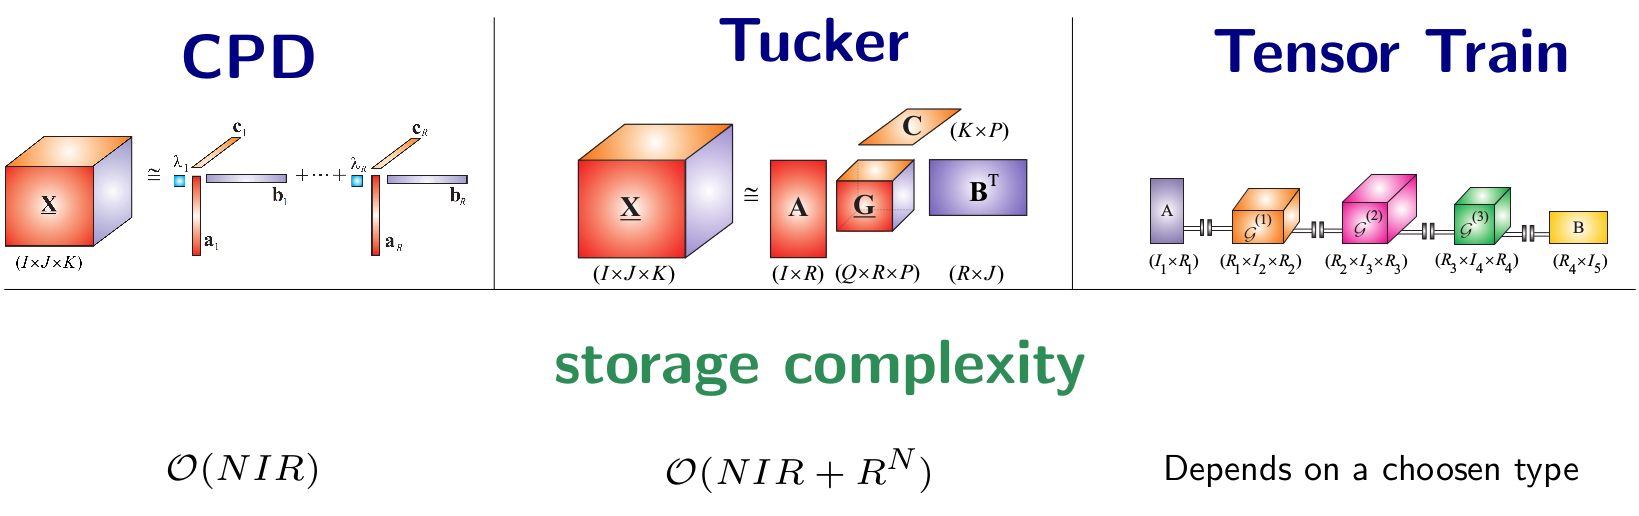
\includegraphics[width = \textwidth]{images/Storage_complexity.png}
    \end{figure}

\end{frame}

%----------------------------------------------------------------------------------------------------------

\begin{frame}{Каноническое представление (CPD)}

    \begin{figure}
        \centering
        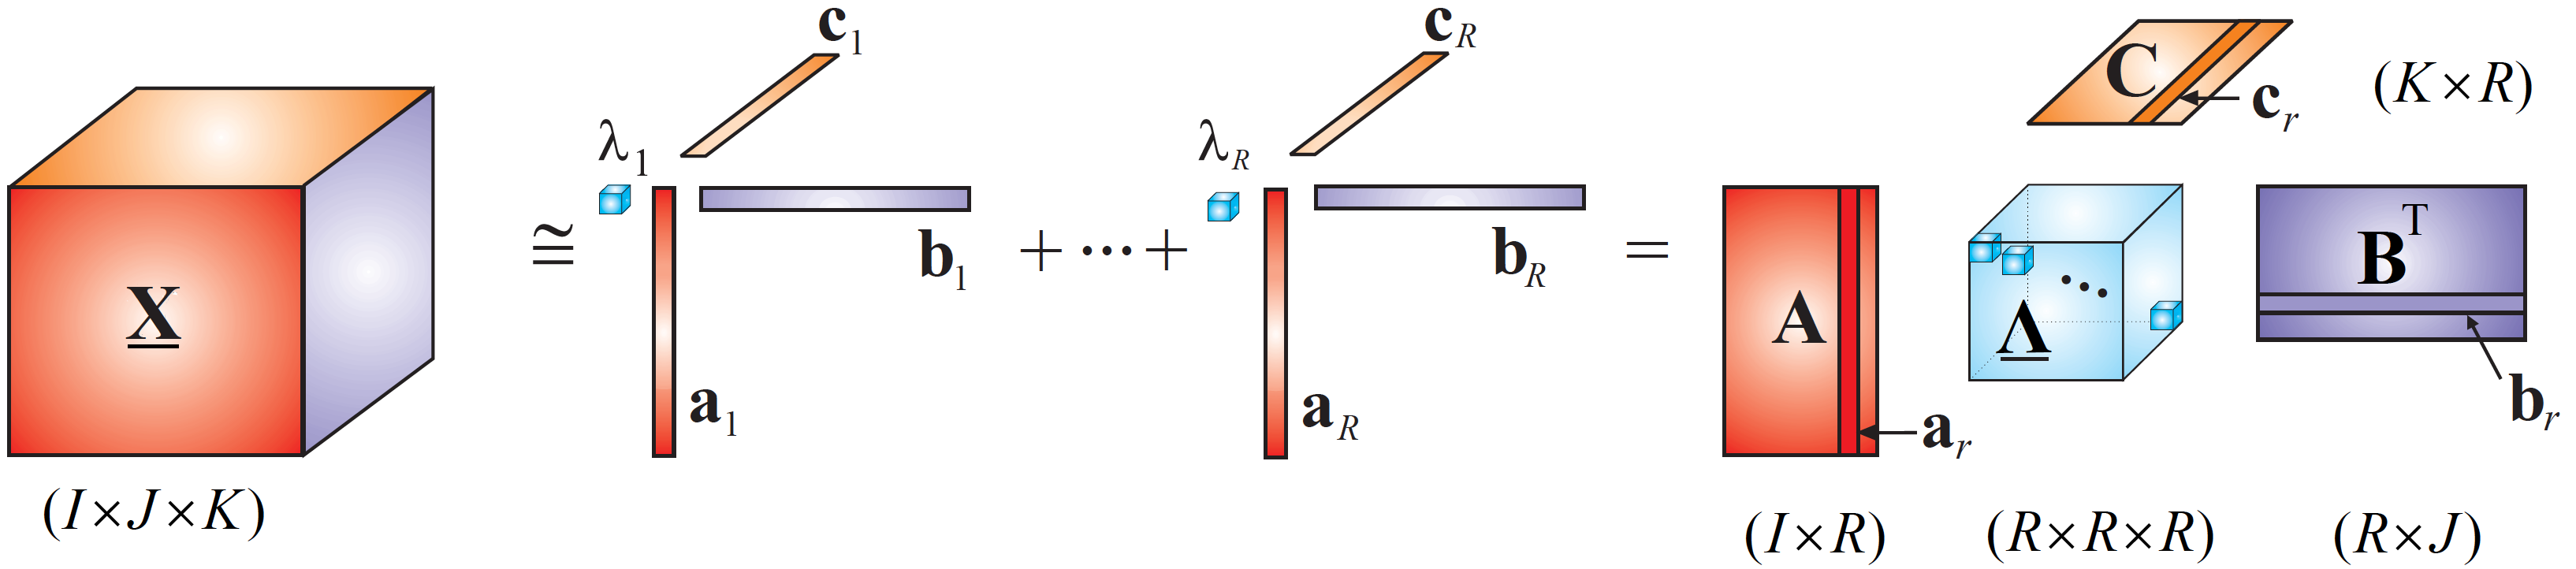
\includegraphics[width = \textwidth]{images/TensorCPD.png}
    \end{figure}


    \begin{align*}
        \mathbf{\underline{X}} \simeq \sum_{r=1}^{R} \lambda_r \mathbf{a}_r \circ \mathbf{b}_r \circ \mathbf{c}_r = \mathbf{\underline{\Lambda}} \times_1 \mathbf{A} \times_2 \mathbf{B} \times_3 \mathbf{C} = \left[    \mathbf{\underline{\Lambda}}; \mathbf{A}, \mathbf{B}, \mathbf{C} \right]
    \end{align*}

\end{frame}

%----------------------------------------------------------------------------------------------------------
\begin{frame}{Представление Таккера (HOSVD, HOOI)}

    \begin{figure}
        \centering
        
\includegraphics[width = \textwidth]{images/TensorTKD.png}
    \end{figure}

    \begin{align*}  
        \mathbf{\underline{X}} \simeq \sum_{q=1}^{Q} \sum_{r=1}^{R} \sum_{p=1}^{P} g_{qrp} \mathbf{a}_q \circ \mathbf{b}_r \circ \mathbf{c}_p = \mathbf{\underline{G}} \times_1 \mathbf{A} \times_2 \mathbf{B} \times_3 \mathbf{C} = \left[    \mathbf{\underline{G}}; \mathbf{A}, \mathbf{B}, \mathbf{C} \right]
    \end{align*}

\end{frame}

%----------------------------------------------------------------------------------------------------------

\begin{frame}{Представление Таккера (HOSVD, HOOI)}

    \begin{enumerate}
        \item Разложение по сингулярным значениям высокого порядка (HOSVD)
            \begin{align*}
                \mathbf{\underline{X}} &= \mathbf{\underline{G}} \times_1 \mathbf{A} \times_2 \mathbf{B} \times_3 \mathbf{C}\\
                \mathbf{X}_{(1)} &= \mathbf{U}_1  \mathbf{\Sigma}_1 \mathbf{V}_1^T \rightarrow \mathbf{A} = \mathbf{U}_1[1:R_1]\\
                \mathbf{X}_{(2)} &= \mathbf{U}_2  \mathbf{\Sigma}_2 \mathbf{V}_2^T \rightarrow \mathbf{B} = \mathbf{U}_2[1:R_2]\\
                \mathbf{X}_{(3)} &= \mathbf{U}_3  \mathbf{\Sigma}_3 \mathbf{V}_3^T \rightarrow \mathbf{C} = \mathbf{U}_3[1:R_3]\\
                \mathbf{\underline{G}} &= \mathbf{\underline{X}} \times_1 \mathbf{A}^T \times_2 \mathbf{B}^T \times_3 \mathbf{C}^T
            \end{align*}
        \item Ортогональная итерация высокого порядка (HOOI)
            \begin{align*}
                &\mathbf{\underline{Y}} = \mathbf{\underline{X}} \times_1 \mathbf{A}^{(1)T} \times_2 \cdots \times_{n-1} \mathbf{A}^{(n-1)T} \times_{n+1} \mathbf{A}^{(n+1)} \times \cdots \times_N \mathbf{A}^{(N)} \\
                &\mathbf{A}^{(n)} \leftarrow R_n \text{ левые сингулярные вектора } \mathbf{Y}_{(n)} \\
                &\mathbf{\underline{G}} = \mathbf{\underline{X}} \times_1 \mathbf{A}^{(1)T}  \times_2 \mathbf{A}^{(2)T} \times_3 \cdots  \times_N \mathbf{A}^{(N)T}
            \end{align*}            
    \end{enumerate}

\end{frame}

%----------------------------------------------------------------------------------------------------------

\begin{frame}{Tензорный поезд (TTSVD)}

    \begin{figure}
        \centering
        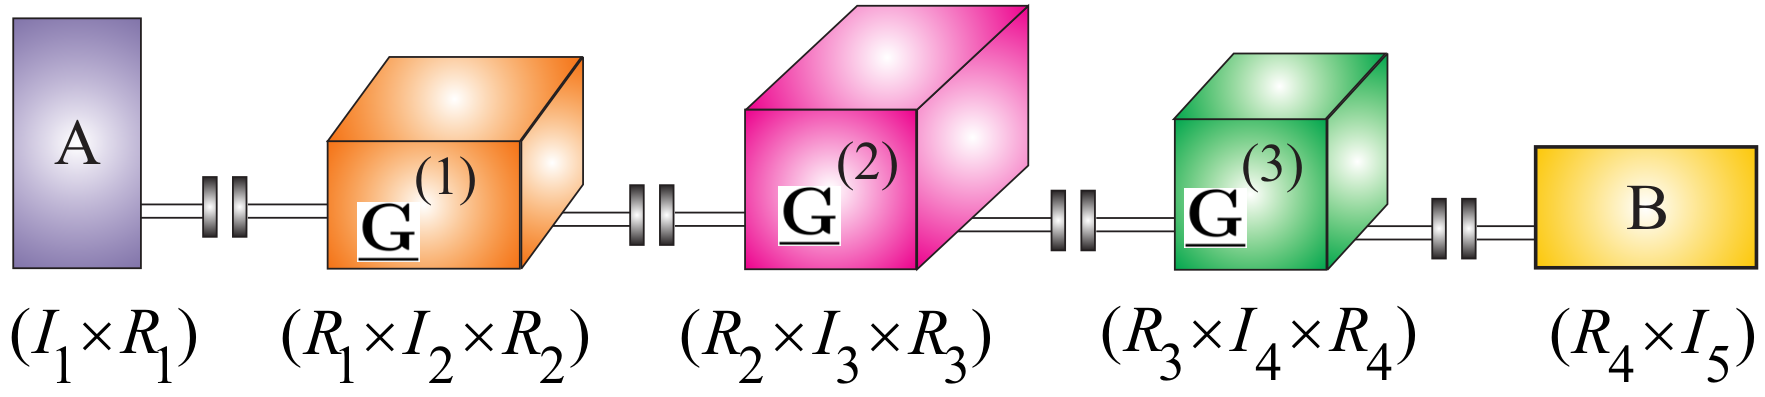
\includegraphics[width = \textwidth]{images/TensorTT.png}
    \end{figure}

    \begin{align*}
        \mathbf{\underline{X}} &= \mathbf{A} \times^1_2 \mathbf{\underline{G}}^{(1)} \times^1_3 \mathbf{\underline{G}}^{(2)} \times^1_3 \cdots \times^1_3 \mathbf{\underline{G}}^{(N-1)} \times^1_3 \mathbf{B} \\
        &= \left[ \mathbf{A}, \mathbf{\underline{G}}^{(1)}, \mathbf{\underline{G}}^{(2)}, \cdots, \mathbf{\underline{G}}^{(N-1)}, \mathbf{B} \right]\\
    \end{align*}

\end{frame}

%----------------------------------------------------------------------------------------------------------

\begin{frame}{Эксперимент}

    Необходимо исследовать в зависимости от разложения:
    \begin{itemize}
        \item Точность
        \item Вычислительную сложность
        \item Устойчивость
    \end{itemize}

    В качестве исследуемого тензора возьмем логотип TensorFlow:

    \begin{figure}
        \centering
        
\includegraphics[width = 0.4 \textwidth]{images/Tensorflow_logo.png}
    \end{figure}
.
  
\end{frame}

%----------------------------------------------------------------------------------------------------------

\begin{frame}{Результат}

    \begin{figure}
        \centering
        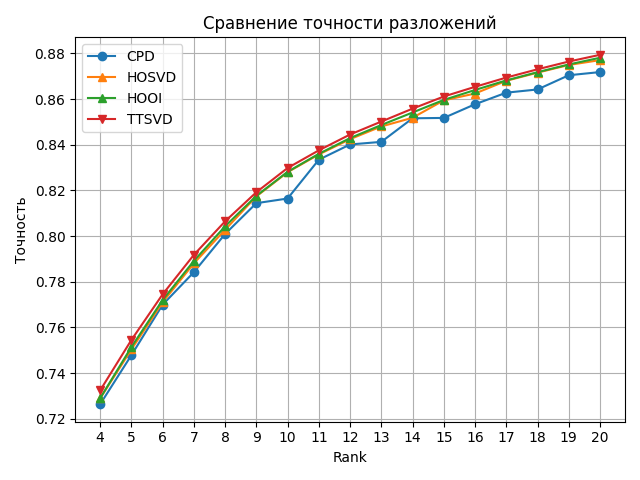
\includegraphics[width = \textwidth]{images/precision.png}
    \end{figure}
  
\end{frame}

%----------------------------------------------------------------------------------------------------------

\begin{frame}{Результат}

    \begin{figure}
        \centering
        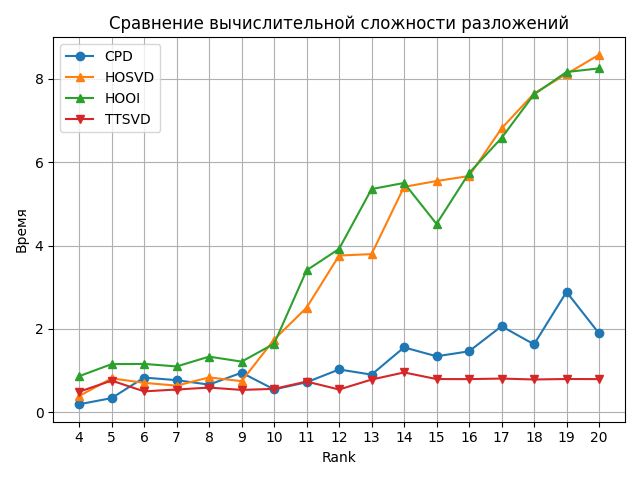
\includegraphics[width = \textwidth]{images/time.png}
    \end{figure}

\end{frame}

%----------------------------------------------------------------------------------------------------------

\begin{frame}{Результат}

    \begin{figure}
        \centering
        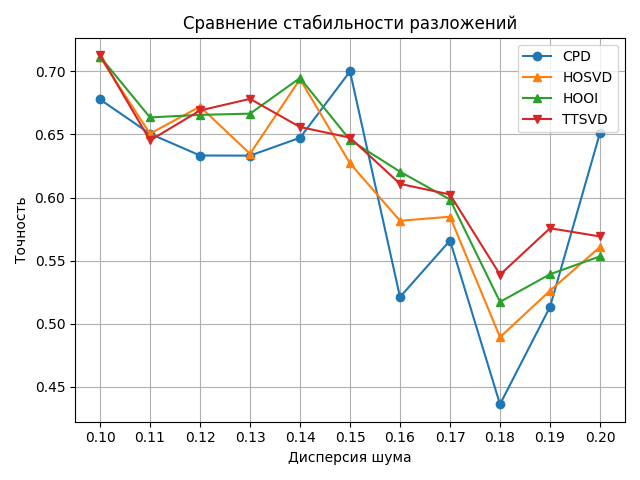
\includegraphics[width = \textwidth]{images/stab.png}
    \end{figure}
  
\end{frame}

%----------------------------------------------------------------------------------------------------------

\begin{frame}{Выводы}
    \begin{itemize}
        \item Были исследованы малоранговые разложения, для которых проведены вычислительные эксперименты, которые показали, что тензорный поезд показывает наилучшие результаты;
        \item Код \url{https://github.com/Dd0-s/Mathematical_forecasting_methods}
    \end{itemize}
\end{frame}

%----------------------------------------------------------------------------------------------------------

\begin{frame}{Литература}

    \begin{enumerate}
        \item \url{https://github.com/hottbox/hottbox};
        \item \url{https://github.com/hottbox/hottbox-tutorials}.
    \end{enumerate}
    
\end{frame}

%-----------------------------------------------------------------------------------------------------

\end{document}